\chapter{Acoplamiento de Modos $p_y$ y Ángulo de Invisibilidad \label{cap:invisibility}}

En electrostática, es posible describir las interacciones dipolares eléctricas mediante los polinomios de Legendre de orden 2, $P_2(\cos\theta) = 3\cos^2\theta - 1$, donde $\theta$ representa el ángulo entre los dipolos. El valor $\theta_m \approx 0.62$ radianes se denomina \textit{ángulo mágico}, ya que anula el término de interacción dipolar \citep{medmagic}.

Este capítulo se centra en los modos dipolares verticales o también llamados modos $p_y$, cuya excitación requiere superar la condición de corte (longitud de onda suficientemente pequeña junto con un contraste $\Delta n$ y un ancho de guía suficientemente grandes).
\section{Acopladores}
Al estudiar el acoplamiento entre modos $p_y$ en guías elípticas, se distinguen dos casos límite: para acopladores horizontales, el acoplamiento $\varkappa_\pi$ presenta signo positivo, mientras que para acopladores verticales, el acoplamiento $\varkappa_\sigma$ tiene signo negativo \cite{Pmodecoupling}.
Este comportamiento es análogo al observado en los enlaces químicos $\sigma$ y $\pi$ de las cadenas de carbono orgánicas. Para verificar este efecto, se fabricaron 20 dímeros con una separación de 25 $\mu$m y una distancia de propagación de 15 mm, variando el ángulo entre guías desde 0.00 rad hasta 1.57 rad. Mediante un modulador espacial de luz (SLM), se generó un modo P caracterizado por dos lóbulos de igual tamaño con una diferencia de fase de $\pi$ entre ellos.
\begin{figure}[H]
    \centering
    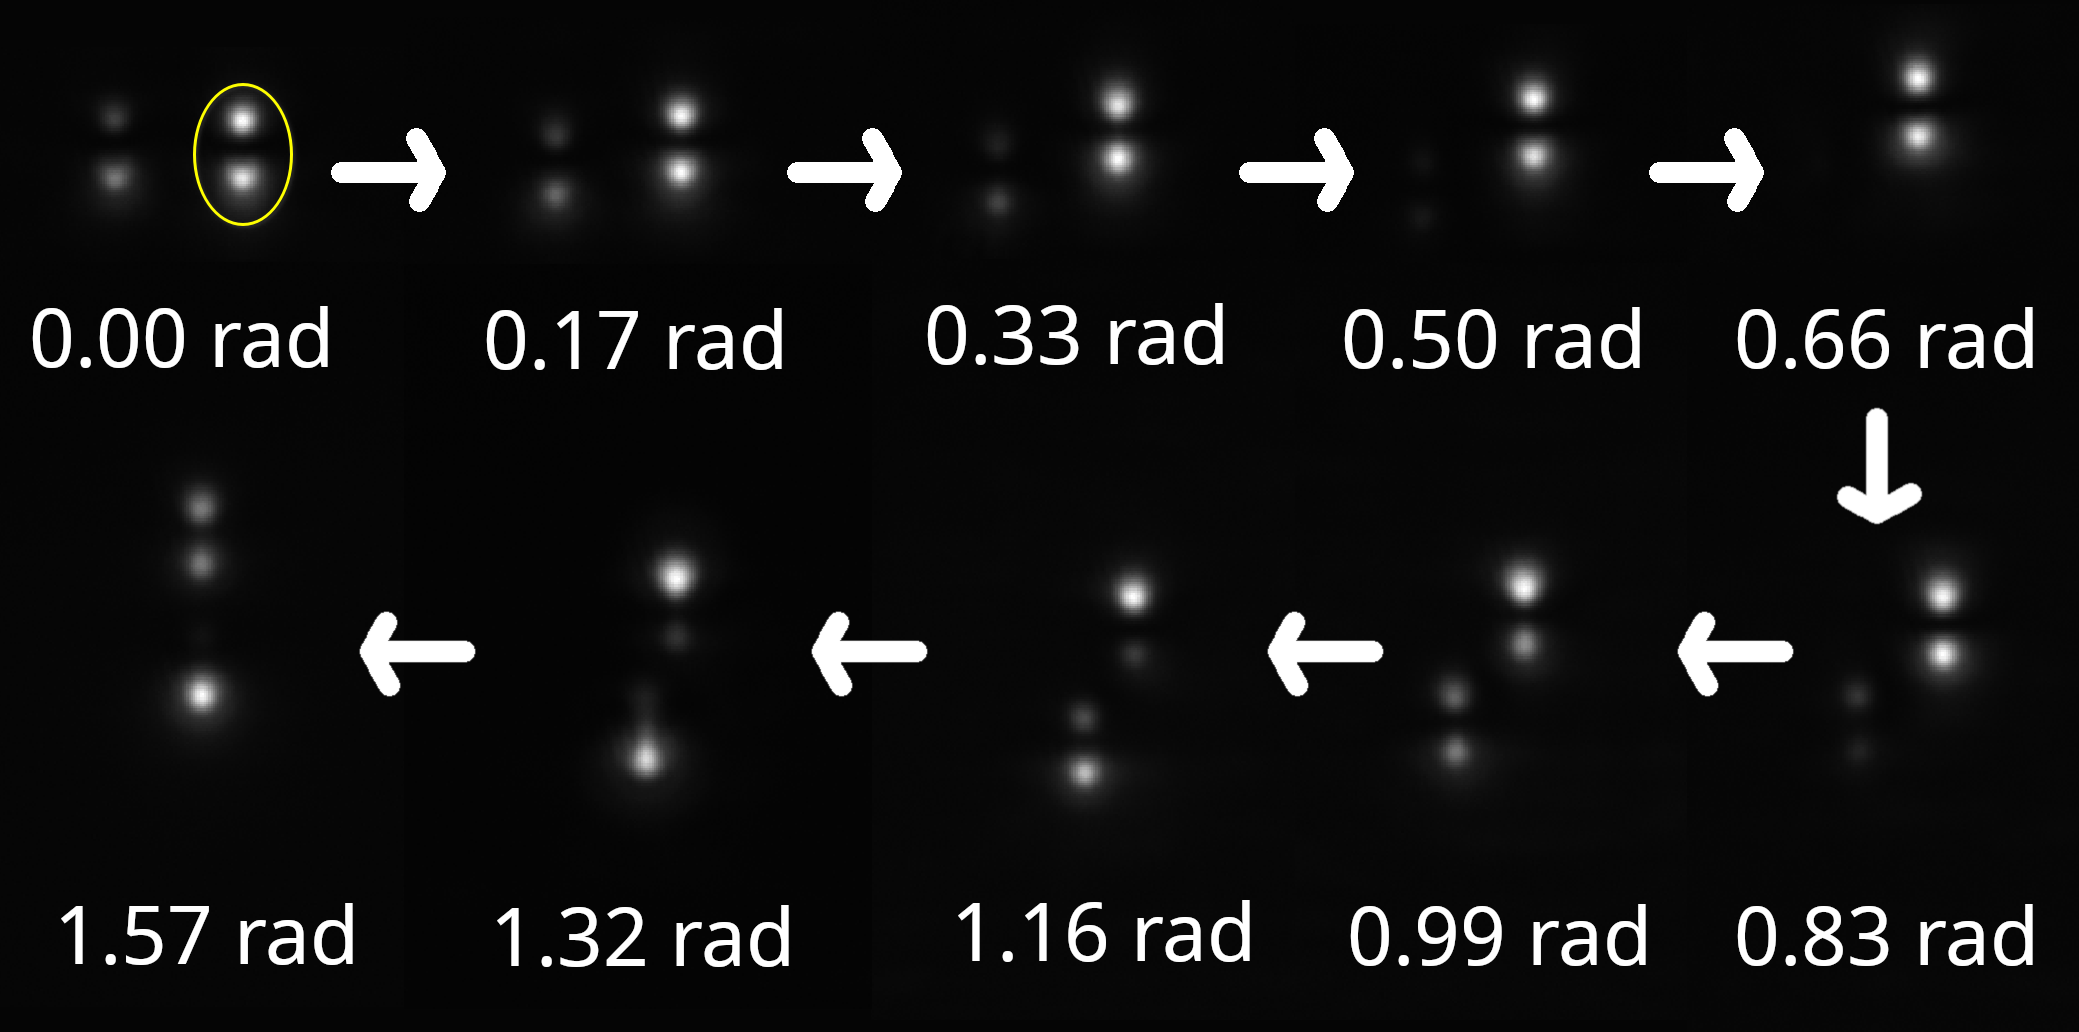
\includegraphics[width=0.7\linewidth]{media/26um_15mm_angles_v2.png}
    \caption[Barrido angular experimental]{Barrido angular experimental para una distancia de propagación de 15 mm. Se observa el efecto del ángulo mágico entre 0.50 y 0.66 rad. \label{fig:angulobarrido}}
\end{figure} \vspace{-2ex} Se analizaron las imágenes siguiendo el método descrito en la Sección \ref{sec:analimag}. Posteriormente, mediante la ecuación (\ref{eqn:coupling-simp}) para el acoplamiento dinámico, se caracterizó su comportamiento en función del ángulo $\theta$ (medido desde la horizontal) para una separación fija de 25 $\mu$m. El signo negativo se introdujo para garantizar la continuidad de la tendencia de los datos, como muestra la Figura \ref{fig:invisibility-coup}.
\begin{figure}[H]
    \centering
    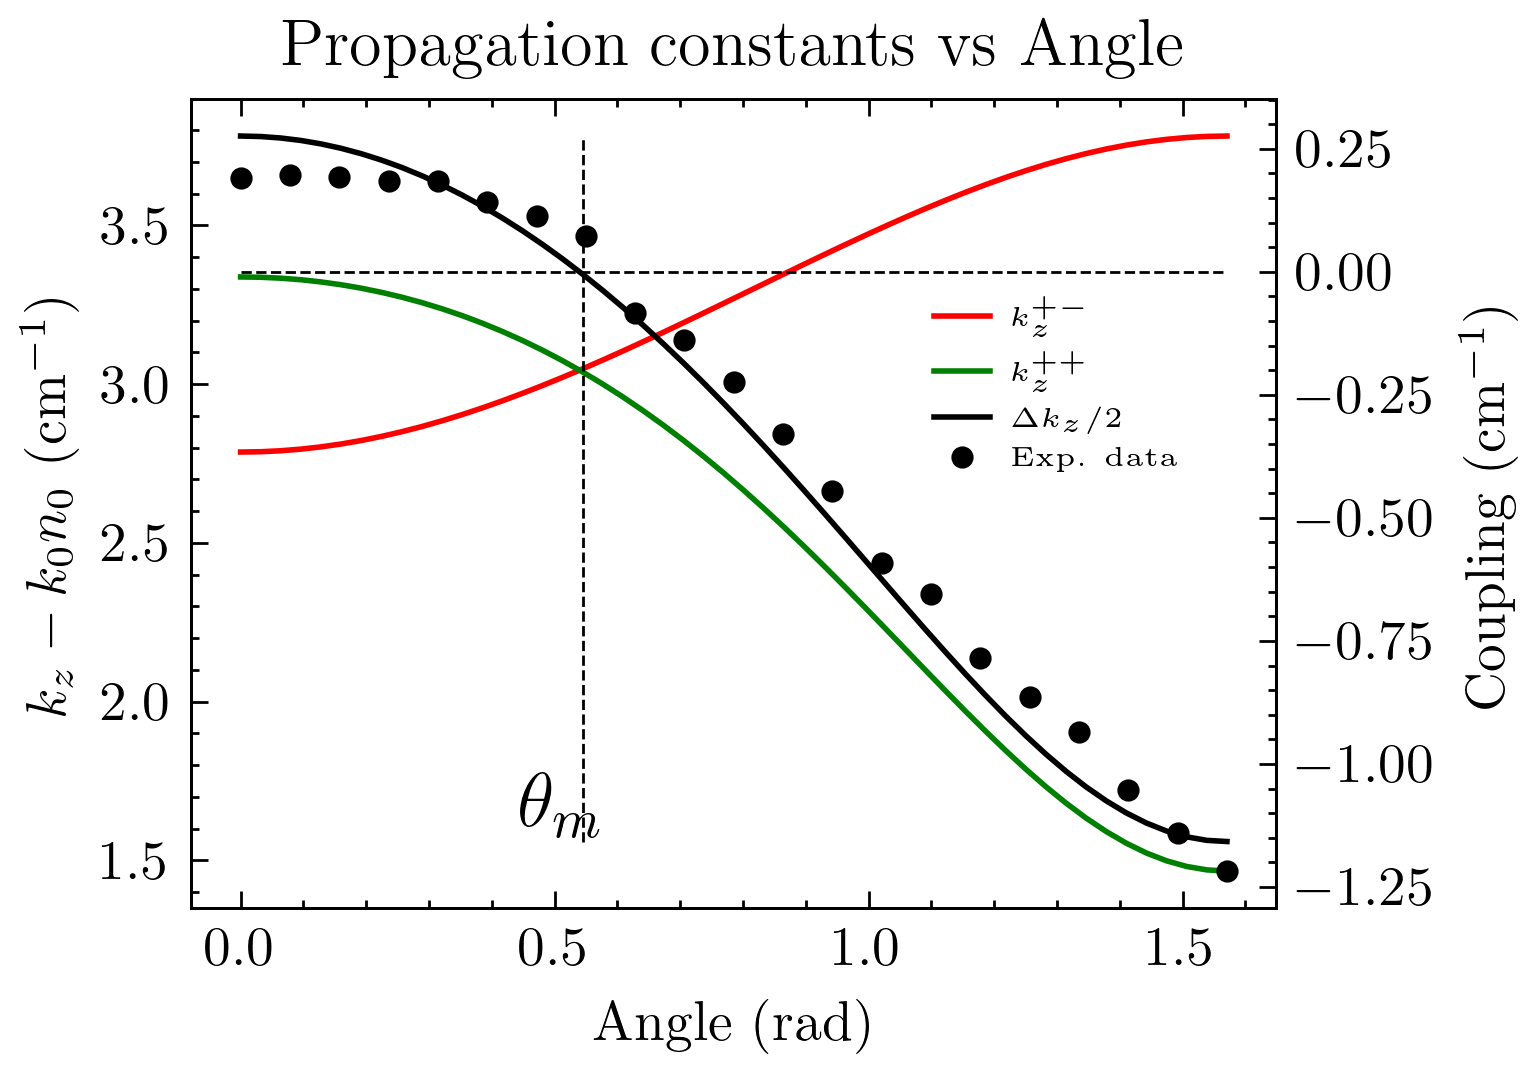
\includegraphics[width=0.6\linewidth]{codigo/eigenvalues_vs_angle.png}
    \caption[Constantes de propagación y acoplamientos angulares para modos P]{Constantes de propagación y acoplamientos en función del ángulo para modos $p_y$, calculados numéricamente mediante EME. Los resultados se comparan con los datos experimentales extraídos de la Figura \ref{fig:angulobarrido}. \label{fig:invisibility-coup}}
\end{figure} \vspace{-2ex}
\section{Redes tipo panal de abeja}
La red tipo panal de abeja, conocida por ser la estructura cristalina subyacente del grafeno, presenta propiedades relevantes para esta tesis, particularmente en sus bandas de Bloch: ambas son dispersivas y exhiben un punto de Dirac \citep{honeycombdirac}. Una vez determinados los parámetros de fabricación en la sección anterior, se estudió el mismo efecto en una red tipo panal de abeja manteniendo constante la distancia entre sitios mientras se variaba el ángulo (Figura \ref{fig:HCLBW}).
\begin{figure}[H]
	\centering
	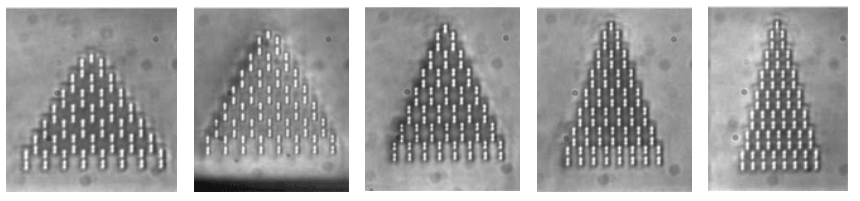
\includegraphics[width=\linewidth]{media/honeycomb_lattices_bw.png}
	\caption[Imágenes de microscopio de redes fotónicas tipo panal de abeja para modos P]{Imágenes de microscopio de redes fotónicas tipo panal de abeja para modos $p_y$ bajo iluminación con luz blanca. \label{fig:HCLBW}}
\end{figure} \vspace{-3ex} Un modelo de primeros vecinos consideraría únicamente el acoplamiento vertical $\varkappa_\sigma$ y el acoplamiento angular $\varkappa_\theta$. Sin embargo, la descripción precisa de los datos experimentales requiere incluir acoplamientos hasta terceros vecinos, así como correcciones por no ortogonalidad. La Figura~\ref{fig:honeycombmodel} muestra un esquema del modelo completo. El Hamiltoniano del sistema se expresa como:
\begin{equation}
	\hat{H}_\Sigma = \hat{H}_{NN} + \hat{H}_{NNN} + \hat{H}_{NNNN},
\end{equation}
donde $\hat{H}_{NN}$, $\hat{H}_{NNN}$ y $\hat{H}_{NNNN}$ contienen los acoplamientos a primeros vecinos ($\varkappa_\sigma$ y $\varkappa_\theta$), segundos vecinos ($t_\pi$ y $t_{\theta 2}$), y terceros vecinos ($t_{\theta 1}$ y $t_{\theta 3}$), respectivamente (ver Figura \ref{fig:honeycombmodel}).

\begin{figure}[H]
	\centering
	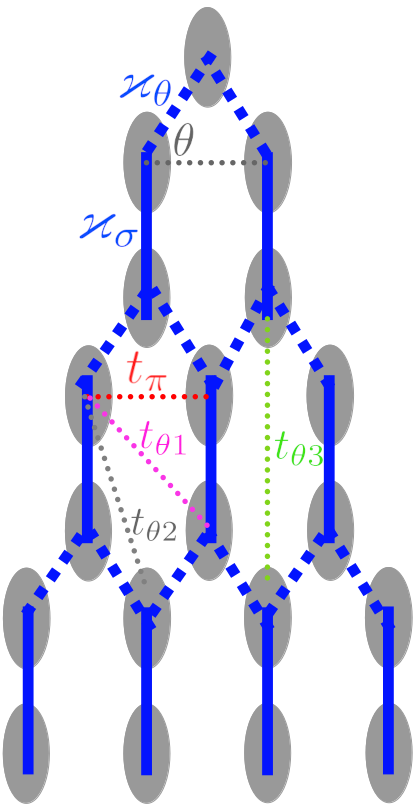
\includegraphics[width=0.25\linewidth]{media/honeycomb-lattice.png}
	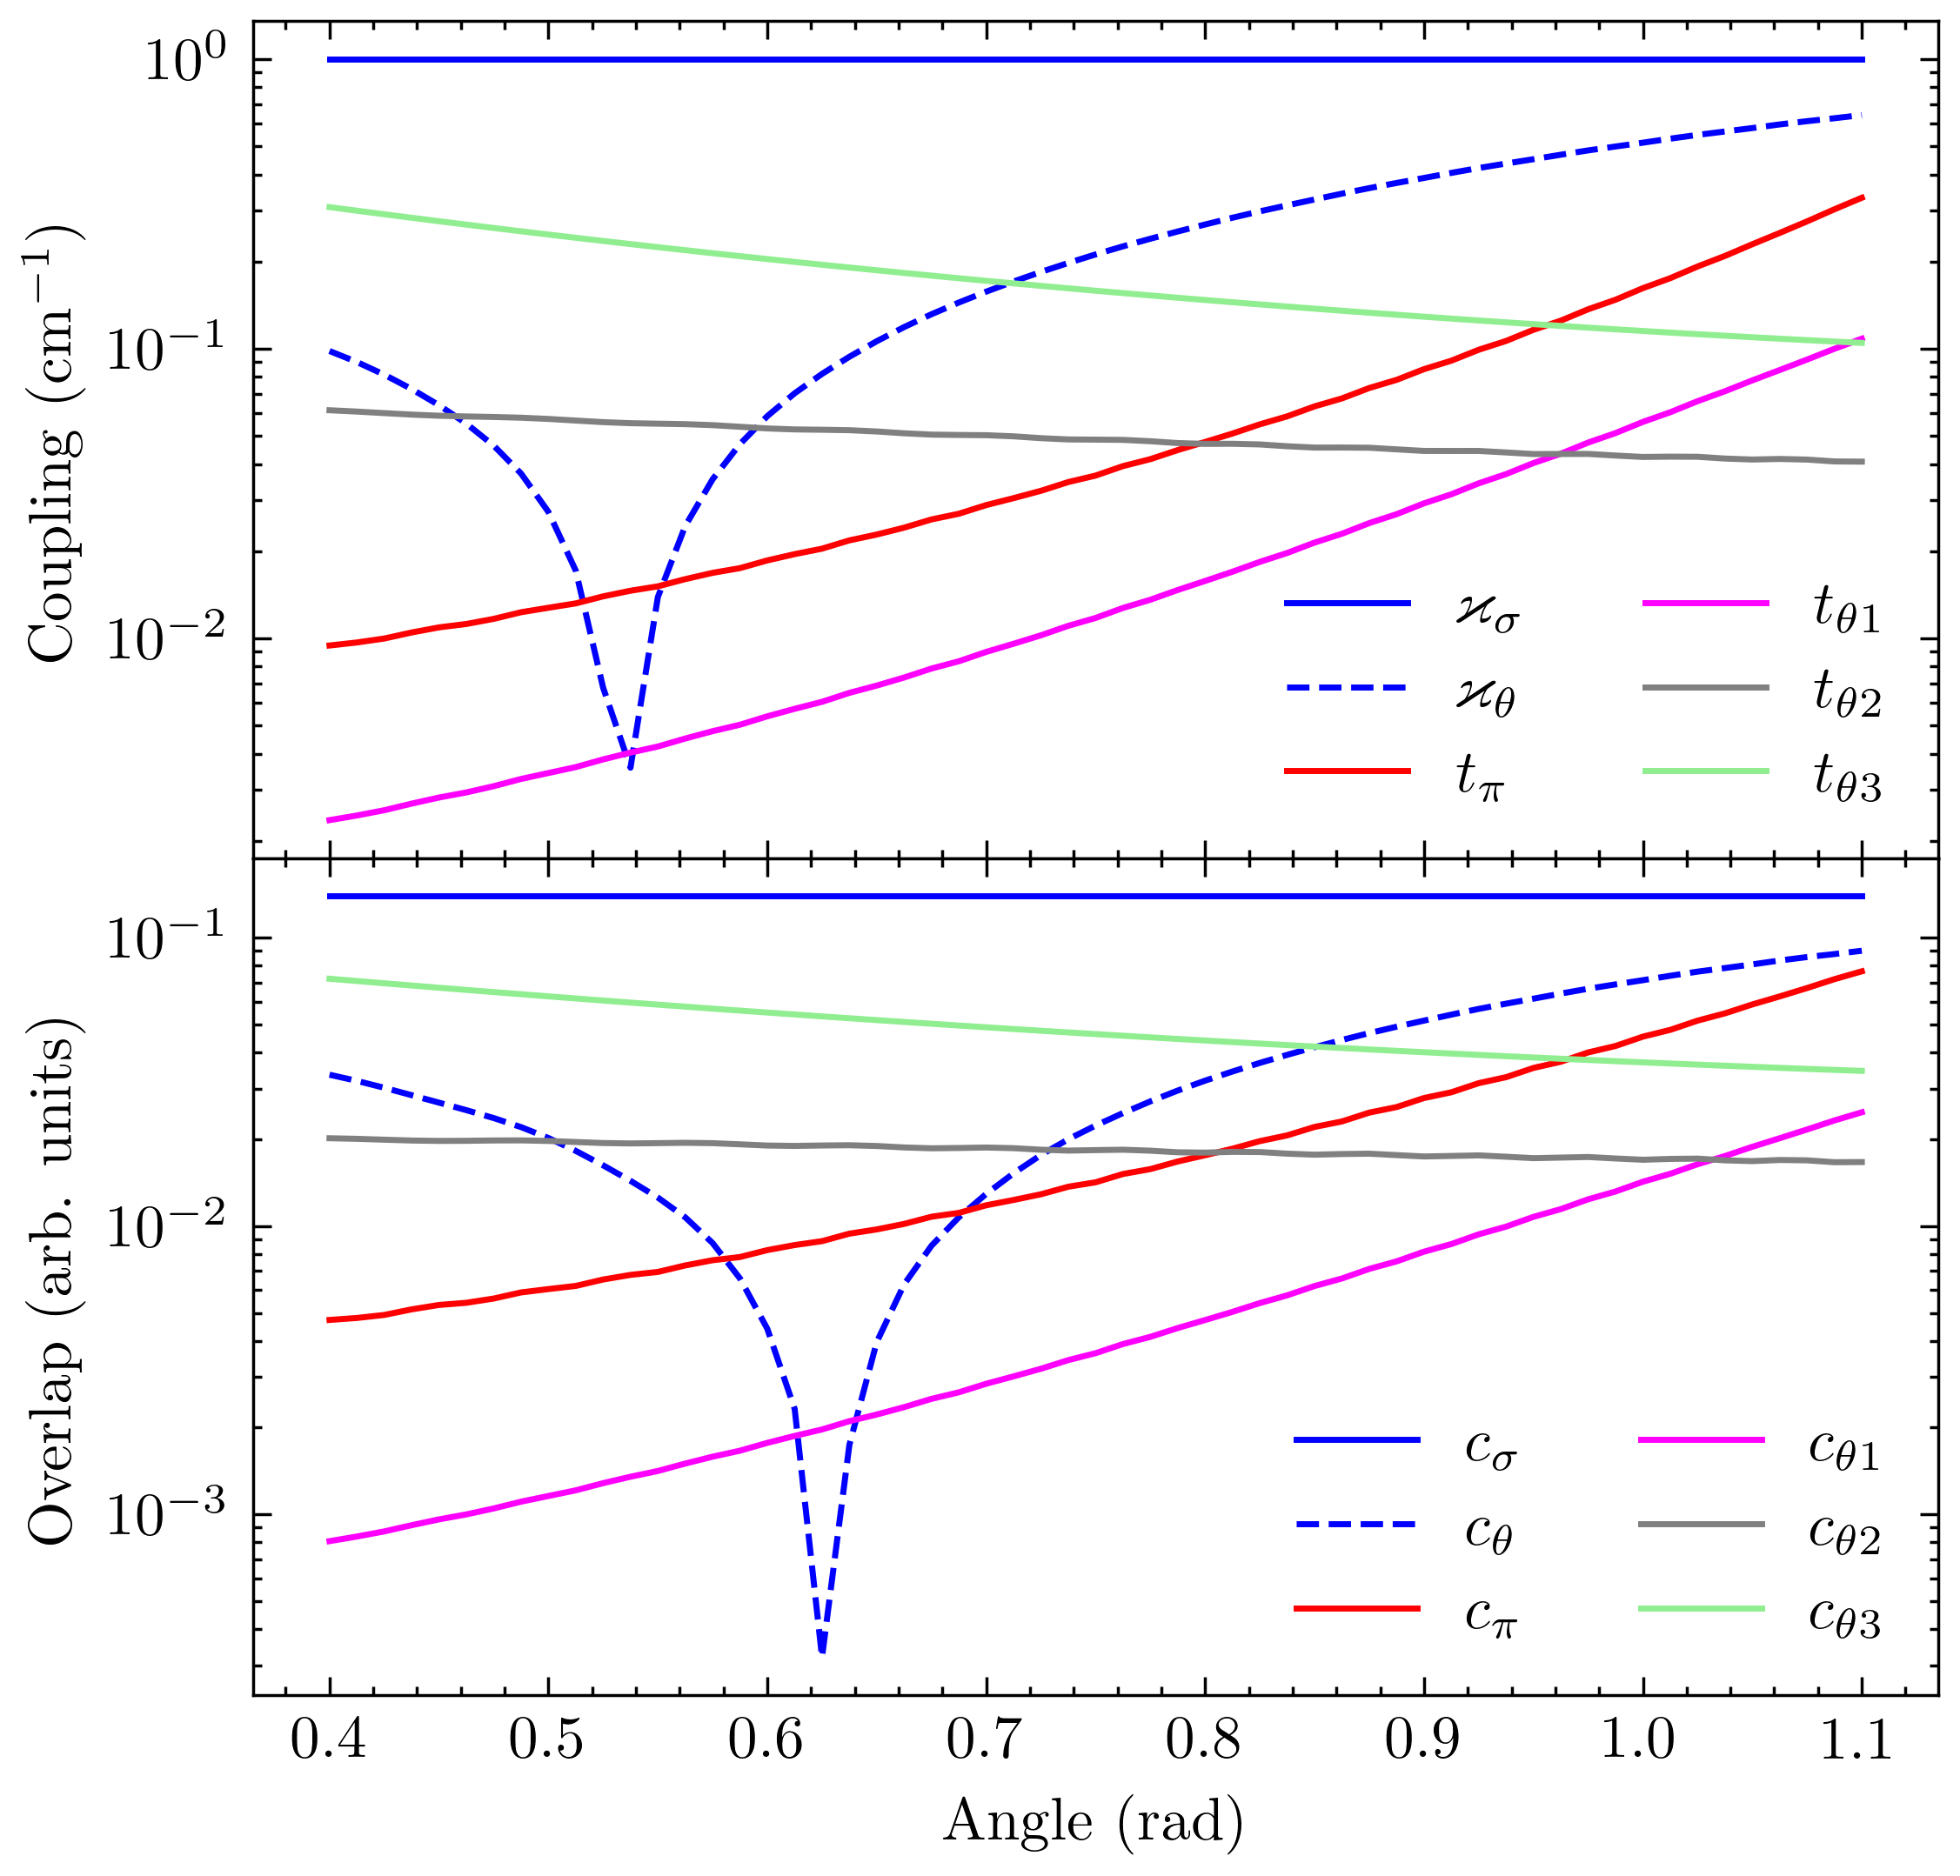
\includegraphics[width=0.55\linewidth]{codigo/NNNN_overlap_vs_angle.png}
	\caption[Modelo de panal de abeja para modos $p_y$ con acoplamientos hasta terceros vecinos]{\textbf{Izquierda:} Esquema del modelo de panal de abeja para modos $p_y$ con acoplamientos hasta terceros vecinos. \textbf{Derecha:} (Arriba) Valores absolutos de los acoplamientos en función del ángulo $\theta$. (Abajo) Integrales de solapamiento normalizadas en función del ángulo $\theta$.\label{fig:honeycombmodel}}
\end{figure} \vspace{-3ex} Además, se define la matriz no ortogonal $\hat{c}$ a partir de la matriz $\hat{P}$ [ecuación~(\ref{eqn:CMTnum})] como $c_{ij} = P_{ij}/I$, donde $I = P_{ii}$ es la intensidad del modo $p_y$, de modo que los elementos diagonales de $\hat{c}$ sean iguales a 1. De manera similar a los acoplamientos, en la Figura \ref{fig:honeycombmodel} se grafica la magnitud de los solapes $c_{ij}$ en función del ángulo.

El Hamiltoniano no hermítico $\hat{H}_\Sigma' \equiv \hat{c}^{-1} \hat{H}_\Sigma$ describe la dinámica de la red e incorpora tanto efectos no ortogonales como acoplamientos de largo alcance. En la Figura \ref{fig:honeycomb-spectra} se muestra el espectro en función del ángulo $\theta$. Se distinguen principalmente dos regiones: una para ángulos $0.4 < \theta < 0.7$, en la que los autovalores se agrupan en tres bandas cuasiplanas, y otra para ángulos $0.7 < \theta < 1.1$, en la que la brecha disminuye en magnitud y, por tanto, se incrementa el transporte en la red. Se calcula el grado de participación inverso (IPR, por sus siglas en inglés) de cada autoestado como $\text{IPR} = \sum_i I_i^2/(\sum_i I_i)^2$. Esto permite la descripción adecuada de los datos experimentales mostrados en el panel derecho de la Figura \ref{fig:honeycomb-spectra}.
\begin{figure}[H]
	\centering
	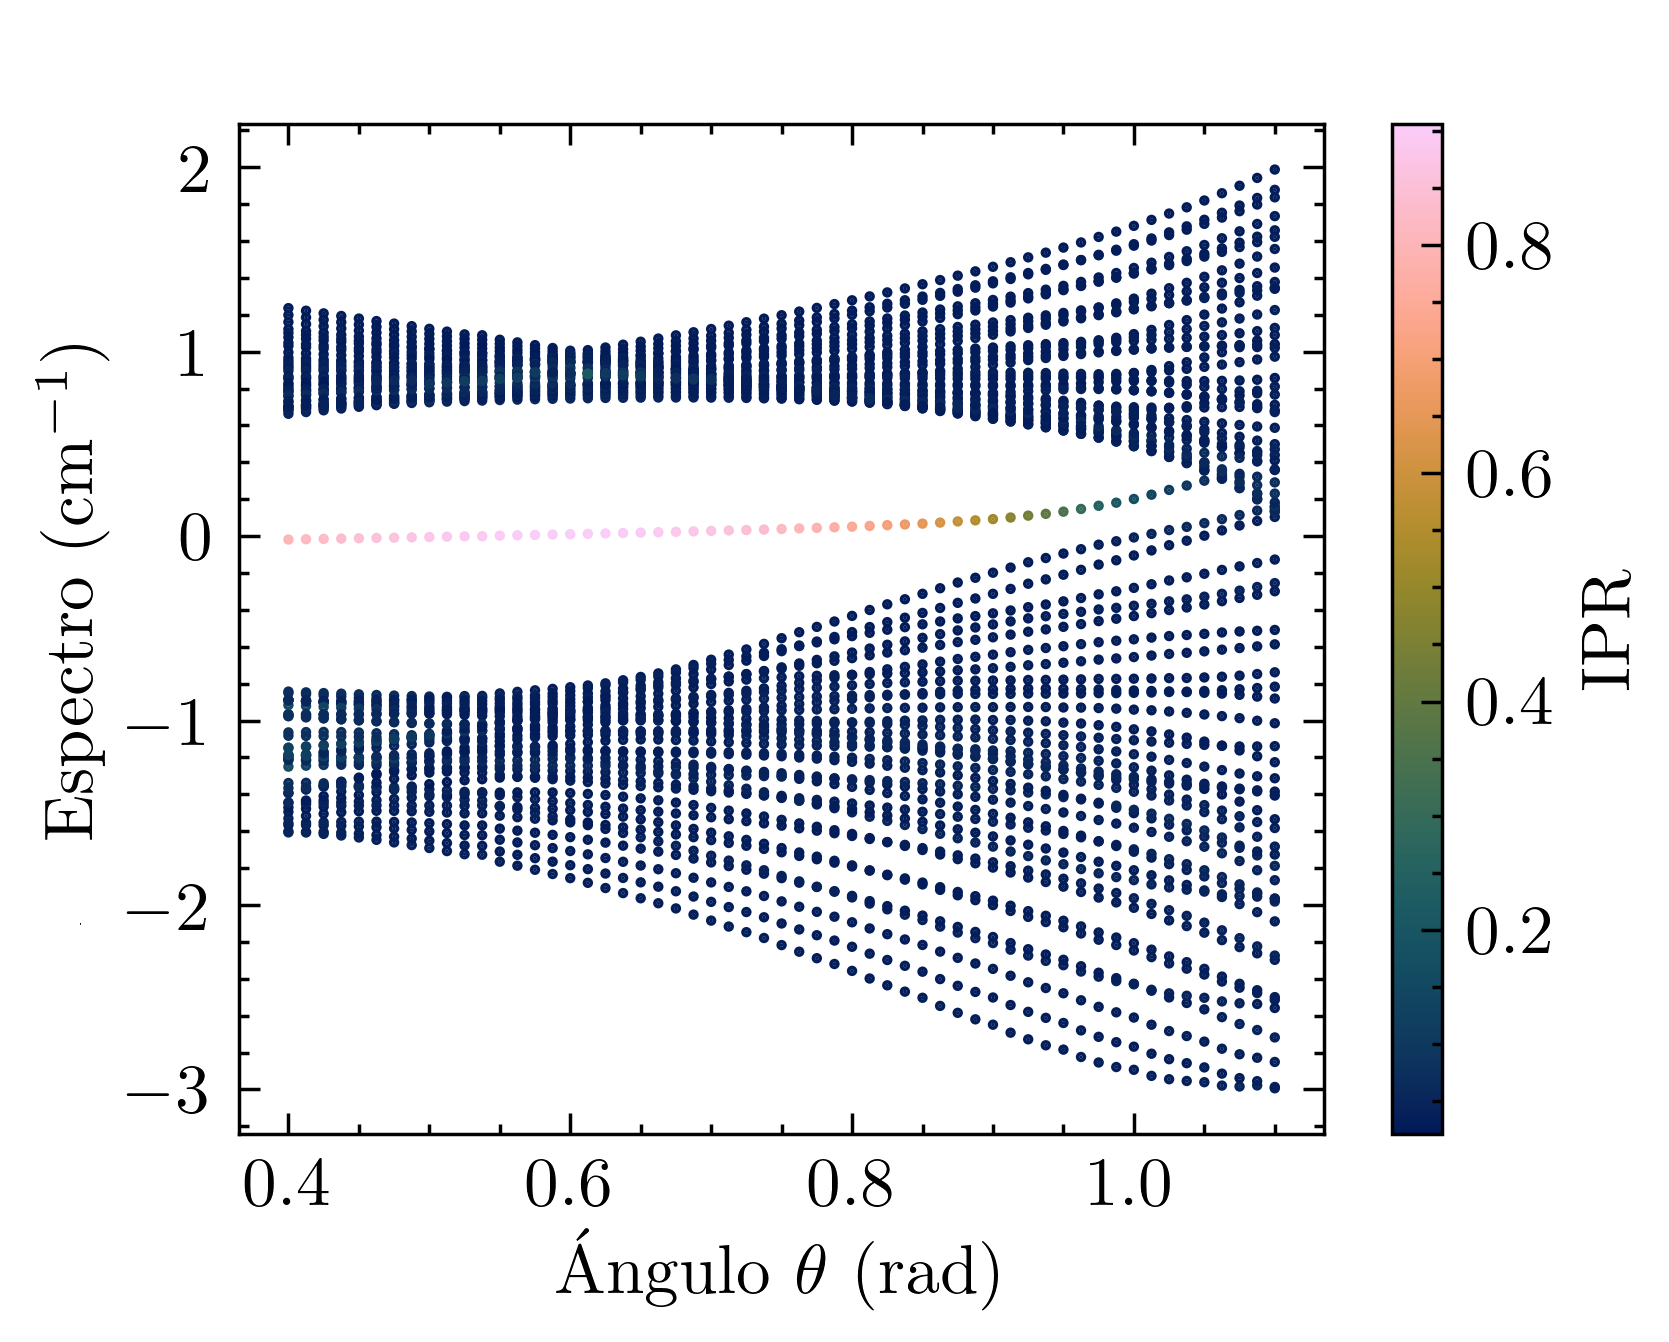
\includegraphics[width=0.45\linewidth]{codigo/honeycomb_eigenvalues_vs_angle.png}
	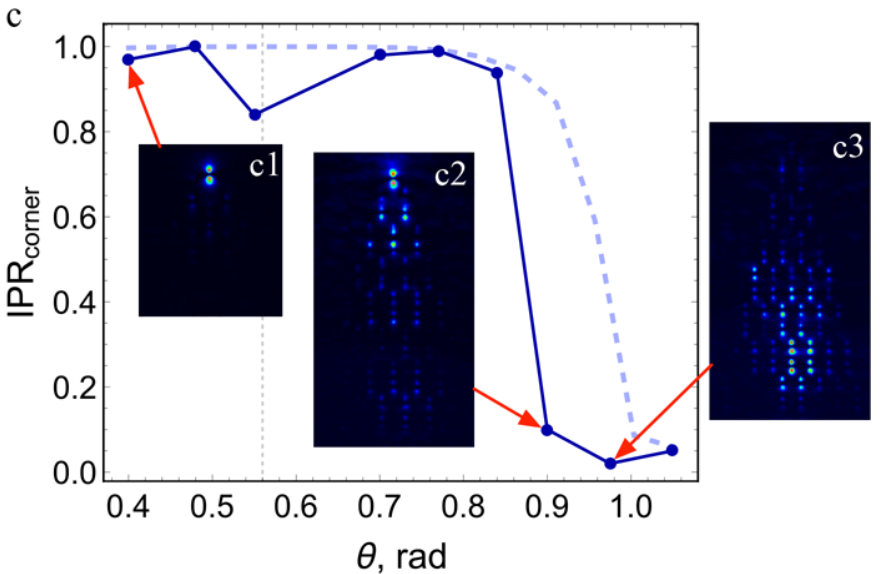
\includegraphics[width=0.5\linewidth]{media/ipr-corner-exp.png}
	\caption[Espectro de la red de panal de abeja de modos $p_y$ en función del ángulo]{\textbf{Izquierda:} Espectro de la matriz $\hat{H}_\Sigma'$ en función del ángulo. Cada punto se colorea según su grado de participación inverso (IPR). \textbf{Derecha:} Grado de participación inverso para la excitación del sitio de esquina en función del ángulo $\theta$.\label{fig:honeycomb-spectra}}
\end{figure} \vspace{-3ex}
La fuerte localización observada al excitar el sitio de esquina se explica porque la proyección de la condición inicial sobre los autoestados corresponde mayoritariamente al autoestado de autovalor nulo. La existencia de este autoestado se debe a la topología que presenta el Hamiltoniano $\hat{H}_\Sigma'$ en el espacio recíproco o de Bloch. Si bien es posible calcular la polarización de bulto mediante bucles de Wilson y determinar que su valor está cuantizado como $\mathbf{P} = (0.5, 0.5)$, resulta más ilustrativo notar que la red puede descomponerse en cadenas cuasi-SSH (ver Figura \ref{fig:cuasi-ssh}). En ambos esquemas, la cuantización es consecuencia de la simetría de inversión presente en la red. 

\begin{figure}[H]
	\centering
	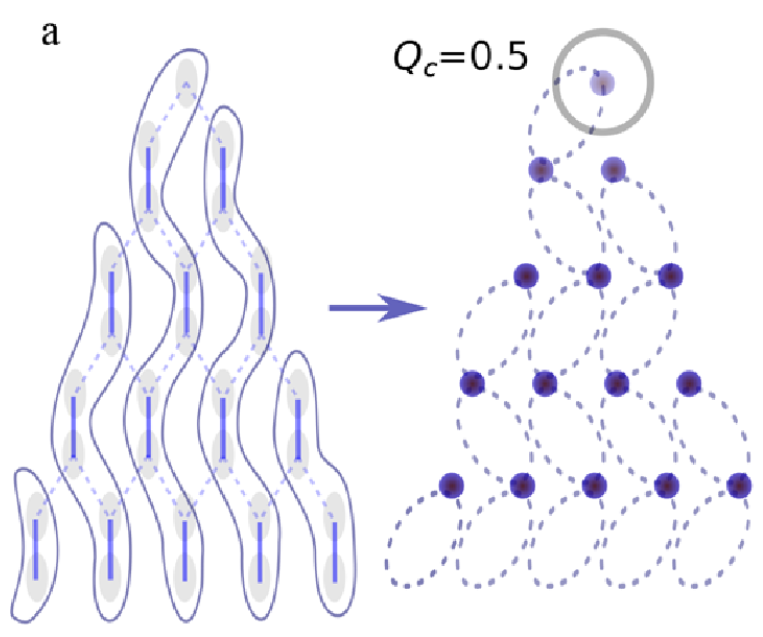
\includegraphics[width=0.5\linewidth]{media/cuasi-ssh.png}
	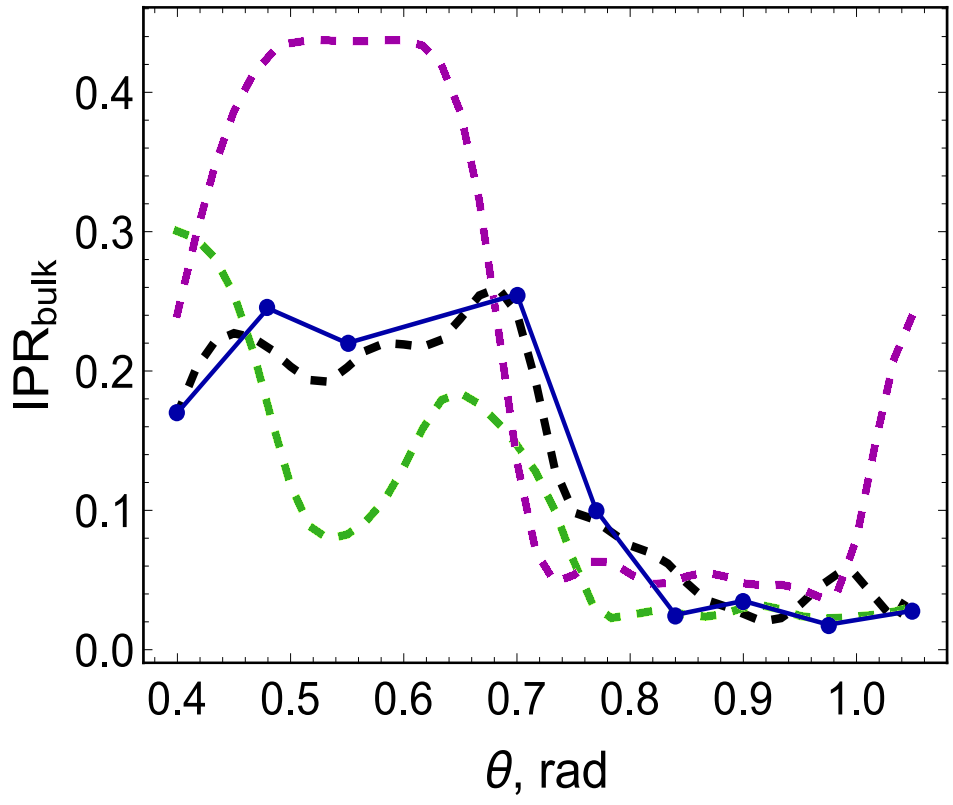
\includegraphics[width=0.45\linewidth]{media/ipr-bulk-exp.png}
	\caption[Descomposición de la red en cadenas cuasi-SSH]{  
		\textbf{Izquierda: }  
		Descomposición de la red en el límite de bandas planas en cadenas SSH de dímeros aislados. \textbf{Derecha: }  IPR para la excitación experimental del sitio central de la red (puntos unidos con líneas para guiar la vista) y simulados numéricamente para tres casos: sin acoplamientos de largo alcance ni correcciones no-ortogonales (curva morada discontinua), con acoplamientos de largo alcance pero sin correcciones no-ortogonales (curva verde discontinua), y con acoplamientos de largo alcance y correcciones no-ortogonales (curva negra discontinua).  \label{fig:cuasi-ssh}}
\end{figure} \vspace{-2ex}
Se estudió experimentalmente la dinámica de bandas planas excitando un único sitio en el bulto de la red para extraer su IPR. Como la excitación inicial en un solo sitio tiene proyecciones no nulas en todas las bandas de Bloch, este experimento magnifica las propiedades dispersivas de las bandas. Así, una propagación casi sin difracción implica un notable aplanamiento de todas las bandas, pues las propiedades de bulto de una red se manifiestan más claramente cuando se excita un sitio central. Un sistema con todas sus bandas planas no exhibiría transporte en la red, limitándose la dinámica únicamente a dímeros efectivos.

Los datos analizados revelan dos regímenes distintos: para redes con $0.4 < \theta < 0.8$ (cercanas al ángulo de invisibilidad) se observa un buen efecto de confinamiento (\emph{caging}). Sin embargo, ángulos mayores ($\theta > 0.8$) favorecen una difracción significativa del campo, resultando en una deslocalización a la salida. Estos resultados experimentales (puntos en Figura \ref{fig:cuasi-ssh}) concuerdan con los cálculos teóricos (línea discontinua). Contrario a lo esperado, los acoplamientos de largo alcance y las correcciones por no ortogonalidad no degradan la dinámica de bandas planas cerca del ángulo de invisibilidad, sino que se complementan. Los valores máximos de IPR ($0.20$-$0.25$) para el estado dímero después de tres ciclos de confinamiento Aharonov-Bohm indican una localización comparable con propuestas ópticas unidimensionales con todas sus bandas planas (ABF). 